\chapter{Конструкторская часть}

В данном разделе будут более подробно рассмотрены выбранные в предыдущем разделе методы и алгоритмы, а также предоставлены требования к программному обеспечению.

\section{Требования к программному обеспечению}
\begin{itemize}[label=\arabic*)]
	\item[-] Возможность отображать заданные сферы с учетом текстуры;
	\item[-] Поддержка различных типов источников света: точечные, направленные и рассеянные;
	\item[-] Учет теней, света и отражений;
	\item[-] Поддержка различных текстурных карт: высот, нормалей, параллактического отображения.
\end{itemize}

\section{Общий алгоритм решения задачи}
\begin{itemize}[label=\arabic*)]
	\item[-] Разместить источники света: определить их позиции и характеристики (типы и интенсивность);
	\item[-] Добавить сферы на сцену;
	\item[-] Загрузить для каждой сферы текстурную карту;
	\item[-] Трассировка лучей и визуализация:
	\begin{itemize}[label=\arabic*)]
		\item[-] Для каждой точки картинной плоскости сгенерировать луч, исходящий из источника наблюдения;
		\item[-] Проанализировать путь луча через сцену, учесть взаимодействия с поверхностью ближайшей сферы;
		\item[-] Внести изменения в нормали сферы с учетом текстурных карт;
		\item[-] Расчитать освещенность, тени и отражения на каждой точке поверхности сферы;
		\item[-] Сформировать окончательное изображение на экране с учетом всех эффектов и модификаций.
	\end{itemize}
\end{itemize}

\section{Трассировка лучей}

В реальном мире свет исходит от источников освещения, отражается от
нескольких объектов и достигает наших глаз. Процесс моделирования пути света называется трассировкой лучей. В компьютерной графике же используются алгоритмы обратной трассировки. Основная идея заключается в анализе путей лучей, исходящих не от источников света, а от “глаз”, смотрящих на предметы. Такой подход соответствует всем привычным нам законам физики, при этом является реальным для реализации, в отличие от симуляции фотонов. [4]

\subsection{Свет}

Для наилучшего отображения реального освещения определим три типа
источников света:
\begin{itemize}[label=\arabic*)]
	\item[-] Точечные источники света: испускают его равномерно во всех направлениях из определенной точки в пространстве;
	\item[-] Направленные источники света: имеют фиксированное направление света, их можно рассматривать как бесконечно удаленные точечные источники, расположенные в заданном направлении;
	\item[-] Рассеянные источники света: привносят часть освещения в каждую точку сцены, независимо от ее положения. Упрощает визуализацию реальной модели, когда свет, достигнув объекта, рассеивает часть обратно в сцену.
\end{itemize}

Таким образом, на сцене мы определим несколько источников света: рассеянные, точечные и направленные.

\subsection{Наблюдатель и сцена}

Первое, что определяется на сцене – положение наблюдателя и окна просмотра. Введем обозначения. Пусть точка $O = (O_{x}, O_{y}, O_{z})$ – позиция камеры. Ширина и высота окна просмотра - $V_{w}, V_{h}$ соответственно. Так же определим расстояние от точки $O$ до плоскости окна – $d$, количество пикселей в окне приложения – $C_{w}$ (по ширине), $C_{h}$ (по высоте) и координаты пиксела на холсте - $C_{x}, C_{y}$.
Для перехода от координат холста ($C_{x}, C_{y}$) к пространственным координатам ($V_{x}, V_{y}, V_{z}$) необходимо будет выполнить следующие преобразования:
\begin{gather}
	V_{x} = C_{x}*\frac{V_{w}}{C_{w}};\hspace{1cm}V_{x} = C_{y}*\frac{V_{h}}{C_{h}};\hspace{1cm}V_{z} = d.
\end{gather}

Итак, для каждой точки холста мы можем определить соответствующую ему точку в окне просмотра.

\subsection{Лучи}

Когда мы определили источник лучей (т. $O$), и их направления ($V$), можно задать луч ($P$). Удобнее всего это сделать с помощью параметрического уравнения:
\begin{gather}
	P = O+t(V-O),
\end{gather}
где $t$ – любое неотрицательное вещественное число. Обозначим направление луча как: $\vec{D}=(V-O)$. Тогда:
\begin{gather}
	P = O+t\vec{D}.
\end{gather}

\subsection{Сферы}

Так как трассировка лучей – трудоемкий процесс, чаще всего вокруг всех
объектов описываются сферы, и проверяется пересечение лучей сначала для них. Таким образом, можно исключить множество ненужных вычислений, и выиграть во времени выполнении программы. Так же, чтобы хранить полную информацию о сфере не нужно так много памяти. Даже не нужно определять сторону для текстуры, поскольку ею будет всегда лишь единственная видимая.

Определим имеющиеся данные о сфере: радиус $r$, и центр $S$. Теперь эти данные необходимо преобразовать, чтобы с ними было удобнее работать.
Пусть точка на поверхности сферы -- $T$. По определению сферы:
\begin{gather}
	\rho(T, S) = r,
\end{gather}
где $\rho$ – расстояние. Оно равно длине вектора:
\begin{gather}
	|T-S| = r.
\end{gather}
Длина вектора – корень из его скалярного произведения с самим собой:
\begin{gather}
	\sqrt{\langle T-S, T-S \rangle} = r;
\end{gather}
\begin{gather}
	\langle T-S, T-S \rangle = r^2.
\end{gather}

\subsection{Пересечение луча и сферы}

Составим систему из имеющихся выражений:
\begin{equation}
	\left\{
	\begin{array}{l}
		\langle T - S, T - S \rangle = r^2 \\
		P = O + t \vec{D}.
	\end{array}
	\right.
\end{equation}

Предположим, что луч и сфера пересекаются, и $T=P$. Остается найти па-
раметр $t$.
Объединим имеющиеся уравнения из формулы (2.8) ($O-S=\vec{SO}$):
\begin{equation}
	\langle \vec{SO}+t\vec{D}, \vec{SO}+t\vec{D} \rangle = r^2.
\end{equation}

Используем дистрибутивность скалярного произведения:
\begin{equation}
	\langle \vec{SO}+t\vec{D}, \vec{SO} \rangle + \langle 	\vec{SO}+t\vec{D}, t\vec{D} \rangle = r^2;
\end{equation}
\begin{equation}
	\langle \vec{SO}, \vec{SO} \rangle + \langle t\vec{D}, t\vec{D} \rangle + \langle t\vec{D}, \vec{SO} \rangle + \langle \vec{SO}, t\vec{D} \rangle = r^2;
\end{equation}
\begin{equation}
	\langle t\vec{D}, t\vec{D} \rangle + 2\langle t\vec{D}, \vec{SO} \rangle + \langle \vec{SO}, \vec{SO} \rangle = r^2.
\end{equation}
Вынесем $t$ за скалярное произведение:
\begin{equation}
	t^2\langle \vec{D}, \vec{D} \rangle + 2t\langle \vec{D}, \vec{SO} \rangle + \langle \vec{SO}, \vec{SO} \rangle - r^2 = 0.
\end{equation}
Мы получили квадратичное уравнение:
\begin{equation}
	at^2+bt+c=0; \hspace*{1cm} \\
	\left\{
	\begin{array}{l}
		a=\langle \vec{D}, \vec{D} \rangle \\
		b=\langle \vec{D}, \vec{SO} \rangle \\
		c=\langle \vec{SO}, \vec{SO} \rangle - r^2.
	\end{array}
	\right.
\end{equation}
Решив его, мы найдем пересечение луча со сферой. Определив пересечение луча со всеми сферами на сцене, мы получим наименьший параметр $t$, который будет соответствовать поверхности, расположенной как можно ближе к
наблюдателю. Ее цвет и надо отобразить. В том случае, если луч не пересек ни одну сферу, мы закрасим пиксел цветом фона.

\subsection{Нормали сферы}

Для вычисления отражений нам понадобится уравнение нормали. Вектор нормали должен быть перпендикулярен поверхности и иметь длину 1, для любой точки сферы он лежит на прямой, проходящей через центр этой сферы:
\begin{equation}
	\vec{N}=\frac{T-S}{|T-S|}.
\end{equation}

\subsection{Диффузное отражение}

Диффузное отражение это процесс, при котором луч света, сталкиваясь с объектом, рассеивается обратно в сцену равномерно во всех направлениях. Именно оно придает матовым объектам матовость.
Рассмотрим луч света с направлением $\vec{L}$ и интенсивностью $I$, который достигает поверхности с нормалью $N$ . Представим интенсивность света как «ширину» луча. Его энергия распределяется по поверхности размером $A$. Отображу ситуацию на рисунке, обозначив вспомогательные углы и точки:

\begin{table}[H]
	\centering
	\begin{tabular}{p{1\linewidth}}
		\centering
		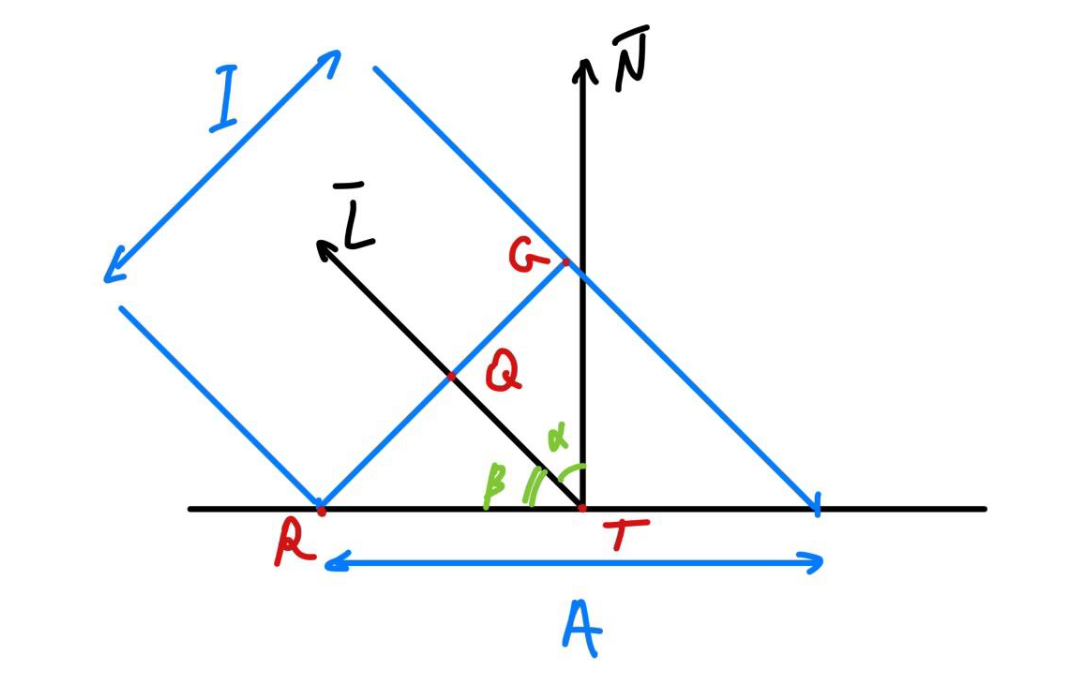
\includegraphics[height=0.4\linewidth]{include/2-1.png}
		\captionof{figure}{Диффузное отражение света}
		\label{img:2-1}
	\end{tabular}
\end{table}

Луч света шириной $I$ достигает поверхности в точке $T$ под углом $\beta$. Нормаль в $T$ это $\vec{N}$ , а переносимая лучом энергия распределяется по поверхности $A$. В случае, когда луч света имеет одинаковое направление с нормалью, $I=A$. С другой стороны, по мере того, как угол между $\vec{L}$ и $\vec{I}$ приближается к 90°, $A\to\infty$. Значит,
\begin{equation}
\lim_{A\to\infty} \frac{I}{A} = 0.
\end{equation}
Выходит, для определения диффузного отражения, нам необходимо узнать что находится на промежутке, выяснив значение $\frac{I}{A}$. Рассмотрим $RG$ – ширину луча. Так как эта прямая перпендикулярна лучу
света, $QRT = \alpha$. В треугольнике $QRT$ сторона $QR=\frac{1}{2}$, а $RT=\frac{A}{2}$. По определению
\begin{equation}
\cos{\alpha}=\frac{QR}{RT}=\frac{\frac{1}{2}}{\frac{A}{2}}=\frac{I}{A}.
\end{equation}
Так как $\alpha$ – угол между $\vec(N)$ и $\vec{L}$, мы можем использовать скалярное произведение этих векторов, чтобы выразить угол как:
\begin{gather}
	\frac{I}{A}=\cos{\alpha}=\frac{\left\langle{\vec{N}, \vec{L}}\right\rangle}{\left| {\vec{N}} \right| \left| {\vec{L}} \right|}.
\end{gather}
Мы получили простое уравнение, дающее нам отражаемую долю света в виде функции угла между нормалью поверхности и направлением света. Если у нас получилось, что значение $\alpha > 90°$, это означает, что свет освещает тыльную сторону поверхности, и учитывать это не нужно.

В итоге, мы можем записать уравнение диффузного отражения для вычисления общего количества света, получаемого точкой $T$ с нормалью $\vec{N}$ в сцене с рассеянным светом с интенсивностью $I_{A}$ и $n$ точечных или направленных источников света с интенсивностью $I_{n}$, а так же световыми векторами $\vec{L_{n}}$:
\begin{gather}
	I_{T} =  I_{A} + \sum_{i=1}^n I_{i}*\frac{\left\langle{\vec{N}, \vec{L}}\right\rangle}{\left| {\vec{N}} \right| \left| {\vec{L}} \right|}.
\end{gather}

\subsection{Зеркальное отражение}

Зеркальное отражение отображает глянцевость объектов. Их вид меняется при смещении точки обзора. Рассмотрим луч света $\vec{L}$ . Нам нужно определить, сколько света от него отражается обратно в направлении точки обзора. Пусть $\vec{V}$ – вектор обзора, указывающий из точки $T$ в сторону камеры, а $\alpha$ – угол между $\vec{R}$ и $\vec{V}$ , тогда получим следующую картину:

\begin{table}[H]
	\centering
	\begin{tabular}{p{1\linewidth}}
		\centering
		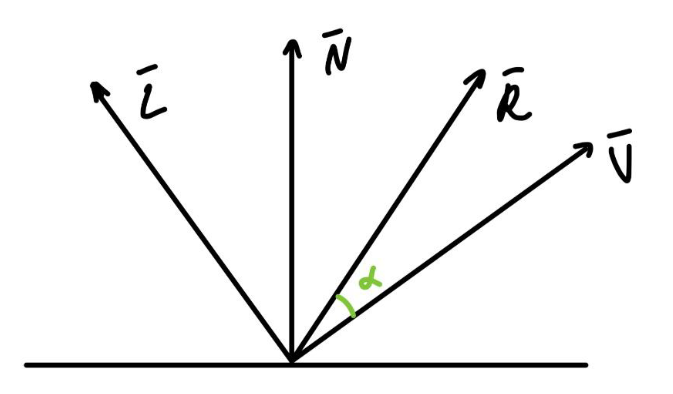
\includegraphics[height=0.3\linewidth]{include/2-2.png}
		\captionof{figure}{Зеркальное отражение света}
		\label{img:2-2}
	\end{tabular}
\end{table}

При $\alpha = 0°$ весь свет отражается в направлении $\vec{V}$ . При $\alpha = 90°$ свет вообще не отражается. Как и в случае с диффузным отражением, нам нужно математическое выражение, позволяющее определить, что происходит при промежуточных значениях $\alpha$.

Данная модель не имеет физического прототипа, но отлично отражает необходимые свойства и проста в вычислении.

Рассмотрим свойство $\cos{\alpha}: \cos{0} = 1 и \cos{\pm90} = 0$. Это мы и будем использовать. Теперь необходимо учесть глянцевость поверхности. Глянцевость – это мера того, как быстро уменьшается функция отражения при возрастании $\alpha$. Простой способ это сделать – возвести $\cos{\alpha}$ в положительную степень $s$:

\begin{table}[H]
	\centering
	\begin{tabular}{p{1\linewidth}}
		\centering
		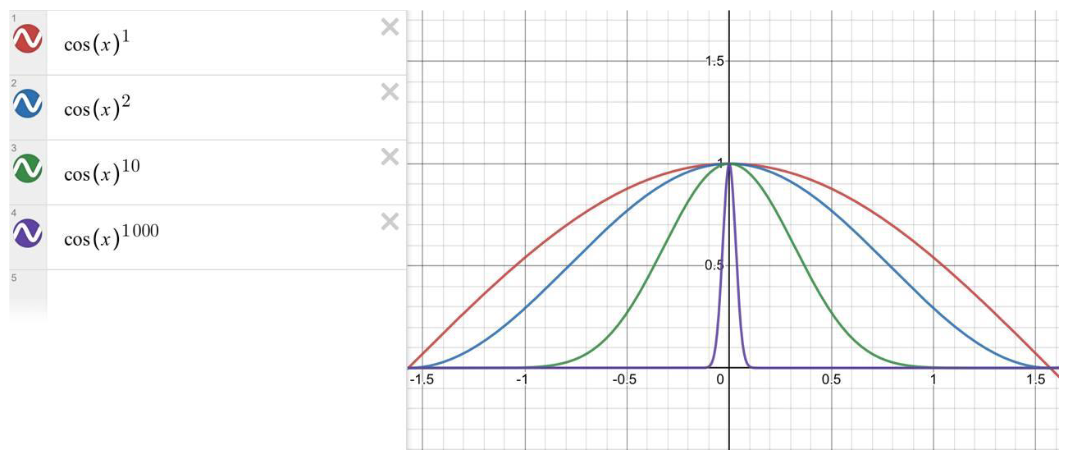
\includegraphics[height=0.4\linewidth]{include/2-3.png}
		\captionof{figure}{График для $\cos{x}^{s}$}
		\label{img:2-3}
	\end{tabular}
\end{table}

$s$ – характеристика блеска поверхности. Для начала вычислим $\vec{R}$ из $\vec{N}$ и $\vec{L}$. Для этого разделим $\vec{L}$ на $\vec{L_{P}}$ и $\vec{L_{N}}$ так, чтобы $\vec{L} = \vec{L_{P}}+\vec{L_{N}}$:

\begin{table}[H]
	\centering
	\begin{tabular}{p{1\linewidth}}
		\centering
		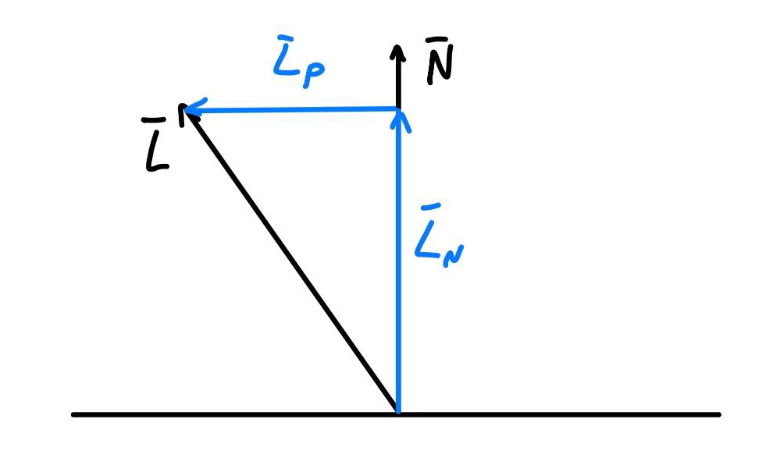
\includegraphics[height=0.3\linewidth]{include/2-4.png}
		\captionof{figure}{Разделение $\vec{L}$ на $\vec{L_{P}}$ и $\vec{L_{N}}$}
		\label{img:2-4}
	\end{tabular}
\end{table}

$\vec{L_{N}}$ – проекция $\vec{L}$ на $\vec{N}$. Исходя из свойств скалярного произведения и того, что длина нормали равняется единице, длина проекции равна $\left\langle{\vec{N}, \vec{L}}\right\rangle$ Так как $\vec{L_{N}}||\vec{N}=\vec{N}*\left\langle{\vec{N}, \vec{L}}\right\rangle$. Получим $\vec{L_{P}}=\vec{L}-\vec{N}*\left\langle{\vec{N}, \vec{L}}\right\rangle$.
Теперь рассмотрим $\vec{R}$:

\begin{table}[H]
	\centering
	\begin{tabular}{p{1\linewidth}}
		\centering
		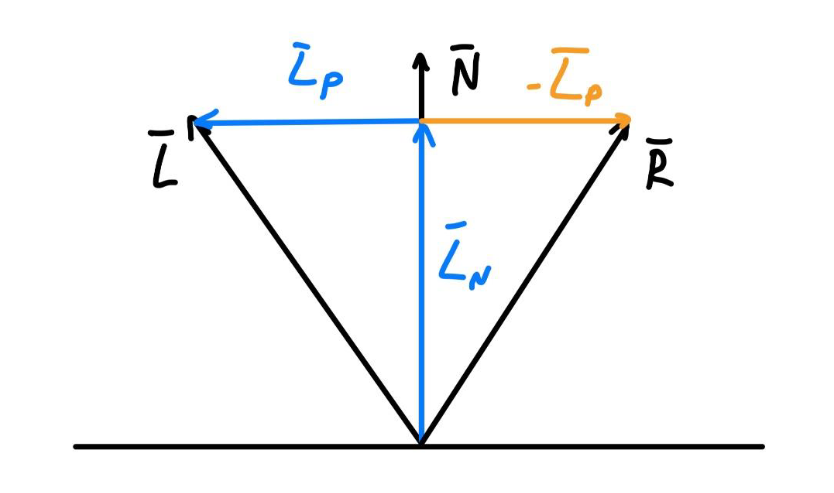
\includegraphics[height=0.3\linewidth]{include/2-5.png}
		\captionof{figure}{Расположение векторов $\vec{R}$ и $\vec{L}$}
		\label{img:2-5}
	\end{tabular}
\end{table}

Исходя из рисунка: $\vec{R} = \vec{L_{N}} -\vec{L_{P}} $. Подставив полученное выше:
\begin{gather}
	\vec{R} = \vec{N}*\left\langle{\vec{N}, \vec{L}}\right\rangle - \vec{L} + \vec{N}*\left\langle{\vec{N}, \vec{L}}\right\rangle = 2*\vec{N}*\left\langle{\vec{N}, \vec{L}}\right\rangle - \vec{L}
\end{gather}
Теперь, по аналогии с диффузным отражением, можно составить уравнение для зеркального:
\begin{gather}
	\vec{R} = 2*\vec{N}*\left\langle{\vec{N}, \vec{L}}\right\rangle - \vec{L};
\end{gather}
\begin{gather}
	I_{S} = I_{L}*\left( \frac{\left\langle{\vec{R}, \vec{V}}\right\rangle}{\left| {\vec{R}} \right| \left| {\vec{V}} \right|} \right)^{S}.
\end{gather}
Как и в случае с диффузным отражением, если $\cos{\alpha}$ оказался отрицательным, его нужно игнорировать. Кроме того, для матовых объектов выражение зеркальности не должно вычисляться. Это можно предусмотреть заранее, пометив соответствующую поверхность, чтобы сократить количество вычислений.

Вычислив зеркальное и диффузное отражение, составим уравнение полного освещения в точке $T$:
\begin{gather}
	I_{T} = I_{A} + \sum_{i=1}^n I_{i}*\left[ {\frac{\left\langle{\vec{N}, \vec{L}}\right\rangle}{\left| {\vec{N}} \right| \left| {\vec{L}} \right|} + \left( \frac{\left\langle{\vec{R}, \vec{V}}\right\rangle}{\left| {\vec{R}} \right| \left| {\vec{V}} \right|} \right)^{S}} \right],
\end{gather}
где $I_{A}$ – интенсивность рассеянного света, $\vec{N}$ – нормаль к поверхности в
точке $T$, $V$ – вектор от $T$ к камере, $s$ – зеркальная характеристика поверхности, $I_{i}$ – интенсивность потока света $u$, $L_{i}$ – вектор из $T$ к свету $i$, а $R_{i}$ – вектор отражения в $T$ для потока света $i$.

\subsection{Тени}

Тени возникают, когда лучи света не могут достичь объекта из-за встреченного на пути препятствия.

Начнем с направленного света. Нам известна точка $T$ на поверхности, а также луч света $\vec{L}$ . Зная это, мы можем определить луч ($O+t\vec{L}$), проходящий из этой точки поверхности к бесконечно удаленному источнику света. Если этот луч пересекается с чем-либо, то точка будет находится в тени и освещения от этого источника нужно игнорировать. В ином случае, мы добавляем освещение данного источника, как было показано ранее.

Точечные источники можно рассматривать так же, но надо учитывать то, что мы не хотим, чтобы объекты дальше источника света могли отбрасывать тени на $T$. Установим $t_{max} = 1$, чтобы при достижении источника света луч останавливался. Так же не стоит забывать, что $t_{min} = eps$, где $aps$ – очень близкое к нулю число справа, чтобы мы не нашли пересечение с поверхностью, из которой и пускаем луч.

\subsection{Отражения}

Когда мы смотрим в зеркало, мы видим отражаемые им лучи света. Они отражаются симметрично относительно нормали поверхности. Итак, нам необходимо выяснить, куда идет луч, отражаемый от зеркальной поверхности.

Таким образом, мы получим рекурсивный алгоритм. При его создании нам нужно убедится, что мы не порождаем бесконечный цикл. У нас будет два условия выхода: когда луч сталкивается с неотражающим объектом, и когда он ни с чем не сталкивается. Также важно вспомнить об эффекте «бесконечного коридора», который образуется, если поставить два зеркала друг напротив друга. Самый простой способ предотвратить бесконечный подсчет отражений: ограничить рекурсию каким-либо числом. В нашей задачи нет необходимости отображать зеркальные поверхности, а тем более визуализировать эффект «бесконечного коридора», поэтому можно обойтись достаточно малым значением в 2-3 единицы.

\section{Связь различных текстурных карт с данными о нормали}

Как было сказано ранее, существует несколько применяемых способов
вносить возмущения в нормали. Рассмотрим соответствующие текстурные
карты от наиболее примитивной, к наиболее сложной.

\subsection{Карты высот (англ. height maps)}

Карты высот имеют черно-белый цвет, что означает, что все каналы RGB (red, green, blue) равны между собой. Таким образом, они хранят единственное значение. Пример:

\begin{table}[H]
	\centering
	\begin{tabular}{p{1\linewidth}}
		\centering
		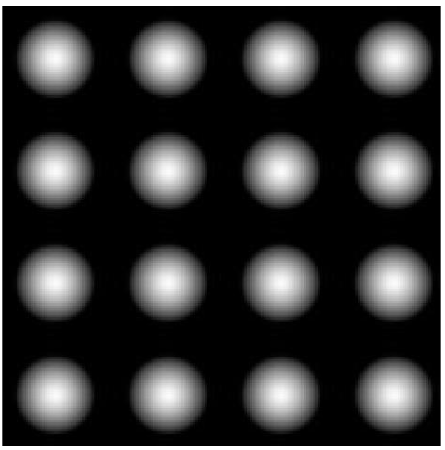
\includegraphics[height=0.3\linewidth]{include/2-6.png}
		\captionof{figure}{Карта высот $h(x, y)$}
		\label{img:2-6}
	\end{tabular}
\end{table}

Чтобы получить возмущение, сначала нужно вычислить аппроксимацию производных по направлениям $x$ и $y$ с помощью разностного аналога [5]:
\begin{gather}
	h_{x}(x, y) = \frac{h(x+1, y) - h(x-1, y)}{2}; \hspace*{1cm} h_{y}(x, y) = \frac{h(x, y+1) - h(x, y-1)}{2}.
\end{gather}

В изображении это будет выглядеть так:
\begin{table}[H]
	\centering
	\begin{tabular}{p{1\linewidth}}
		\centering
		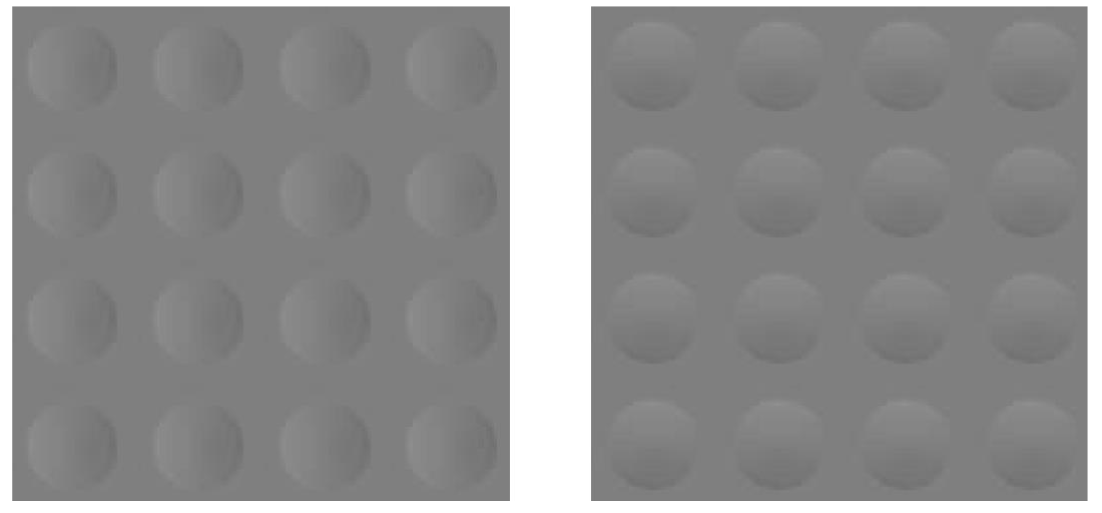
\includegraphics[height=0.3\linewidth]{include/2-7.png}
		\captionof{figure}{Аппроксимация по $x$ (слева) и $y$ (справа)}
		\label{img:2-7}
	\end{tabular}
\end{table}

Тогда ненормализованное значение нормали в текстеле $(x, y)$:
\begin{gather}
	N'(x, y)=(-h_{x}(x, y) - h_{y}(x, y), 1).
\end{gather}

\subsection{Карты нормалей (англ. normal maps)}
Карты нормалей содержат значения в двух каналах. Принято хранить $h_{x}$ в
канале R, а $h_{y}$ в G. Тогда значение канала B не используется, и все карты имеют голубоватый оттенок

В изображении это будет выглядеть так:
\begin{table}[H]
	\centering
	\begin{tabular}{p{1\linewidth}}
		\centering
		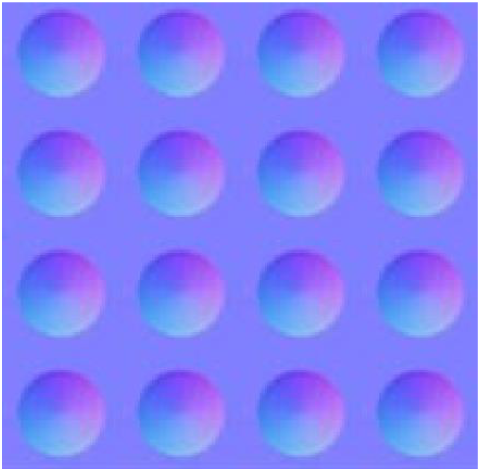
\includegraphics[height=0.3\linewidth]{include/2-8.png}
		\captionof{figure}{Карта нормалей}
		\label{img:2-8}
	\end{tabular}
\end{table}

\subsection{Карта параллактического отображения (англ. parallax map)}
С предыдущими типами карт есть проблема: при смещении угла обзора, это никак не влияет на рельеф. Если мы посмотрим вдоль реальной кирпичной стены под некоторым углом, мы не увидим зазор между кирпичами. Это происходит, потому что мы лишь изменяли нормали.

Идея параллакса заключается в том, что положение объектов относительно друг друга должно изменятся с движением наблюдателя. Неровности должны увеличиваться в высоту [5].

\begin{table}[H]
	\centering
	\begin{tabular}{p{1\linewidth}}
		\centering
		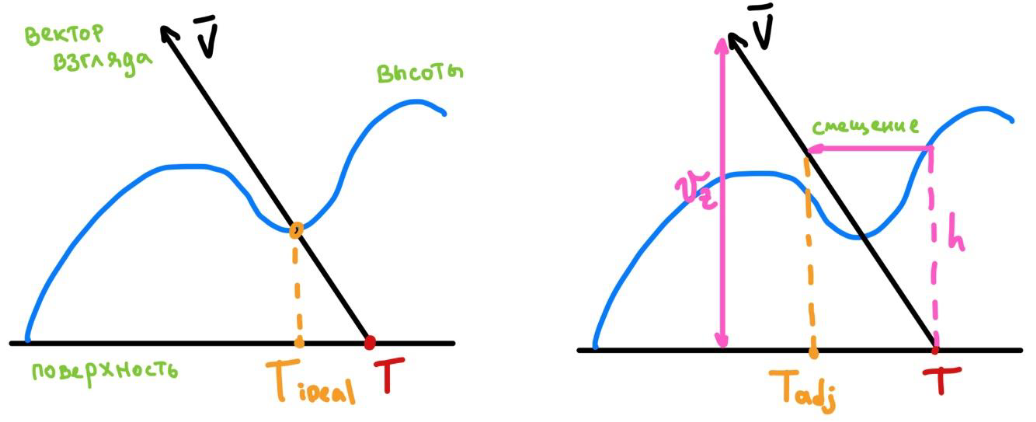
\includegraphics[height=0.3\linewidth]{include/2-9.png}
		\captionof{figure}{Фактическое положение поверхности определяется лучом взгляда (слева). Параллактическое отображение выполняет аппроксимацию, используя высоту для нахождения положения новой точки (справа).}
		\label{img:2-9}
	\end{tabular}
\end{table}

Теперь, помимо направления нормали, нам необходимо хранить высоту $h$. Учитывая местоположение с координатами текстуры $T$, высоту $h$, нормализованный вектор вида $V$ со значением высоты $V_{z}$ и горизонтальной составляющей $V_{xy}$, новая скорректированная по параллаксу текстурная координата:
\begin{gather}
	T_{adj} = T + \frac{h*V_{xy}}{V_{z}}.
\end{gather}
Однако, когда вектор обзора находится вблизи горизонта поверхности, небольшое изменение высоты приводит к большому смещению координат текстуры. Аппроксимация не будет корректной, поскольку полученное новое местоположение практически не коррелирует по высоте с исходным местоположением на поверхности. Чтобы решить эту проблему, мы может ограничить смещение: оно не должно превышать высоту. Тогда уравнение будет иметь вид:
\begin{gather}
	T_{adj} = T + h*V_{xy}.
\end{gather}
При крутых углах, это уравнение почти совпадает с исходным, поскольку $V_{z} \approx 1$. При малых углах смещение становится ограниченным. Но даже с такими ограничениями параллактическое смещение должно обеспечивать более реалистичное представление.

\section{Наложение текстуры на поверхность}

Теперь, когда у нас есть все необходимые уравнения и преобразования, остается лишь связать текстурную карту с поверхностью. То есть нужно определить, какой пиксел $h_{xy}$ текстурной карты соответствует точке на сфере. Определим
\begin{gather}
	x=u*M_w; \hspace*{1cm} y=v*M_h,
\end{gather}
где $M_w, M_h$ -- угол между положительным направлением оси $x$ и проекцией нормали к поверхности сферы на плоскость $XY$. Его мы можем вычислить по следующей формуле:
\begin{gather}
	\phi=\arctan{\frac{N_y}{N_x}}.
\end{gather}
Этот угол измеряет поворот вокруг вертикальной оси $Z$ на плоскости $XY$. Он учитывает вращение окружности вокруг вертикальной оси, что является сферой. Переведя этот угол в диапазон $[0, 1]$ получим необходимое значение $u$:
\begin{gather}
	u=\frac{\phi+\pi}{2\pi}.
\end{gather}
Пусть $\theta$ -- угол между нормалью и положительным направлением оси $Z$:
\begin{gather}
	\theta=\arccos{N_z}.
\end{gather}
Данный же угол определяет наклон нормали относительно вертикальной оси. На сфере он соответствует углу между нормалью и радиус-вектором точки на сфере. Он позволяет корректно распределить текстуру вдоль вертикальной оси сферы. Остается привести угол в необходимый диапазон, получив $v$:
\begin{gather}
	v=\frac{\theta}{\phi}.
\end{gather}

\section{Схема алгоритма трассировки луча}
\begin{table}[H]
	\centering
	\begin{tabular}{p{1\linewidth}}
		\centering
		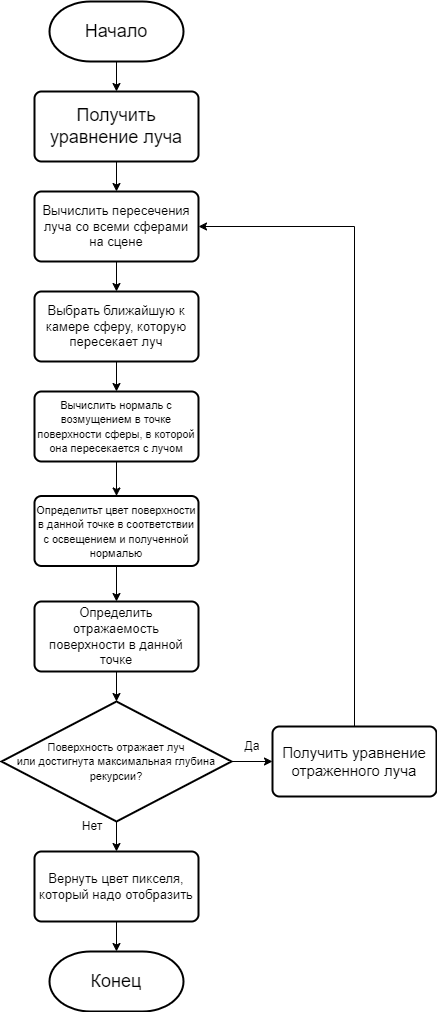
\includegraphics[height=1\linewidth]{include/2-10.drawio.png}
		\captionof{figure}{Блок-схема алгоритма трассировки луча.}
		\label{img:2-10}
	\end{tabular}
\end{table}

\section*{Вывод}

В данном разделе были подробно рассмотрены алгоритмы, необходимые для реализации поставленной цели.